\newpage
\subsection{The Transforming Masking method}
\label{The_Transforming_Masking_Method}


Here is presented in detail for the DES algorithm an important counter-measure, 
called Transformed Masking Method presented 
\footnote{Patterned and deprecated countermeasure !!}
by M-L.Akkar and C.Giraud at the CHES'2001 \nocite{ches-2001}
\cite{phd-Giraud-2007}, 


%see also \cite{fse-2003-akkar} and
% \cite{ches-2001-akkar}.


\begin{center}
"what does prevent an programmer to effectively mask the intermediate values\\ 
by xoring the plaintext, M, with a random mask, R, without changing the cyphertext??"

the S-boxes !
\end{center}

\subsubsection{General principle}
Recall that in the NIST specification $IP$ stands for the initial 
bijection of the DES, $FP$ for the final one -inverse of the $IP$-,
$EP$ stands the compressive function (surjection) at the beginning
of the $f$-function and $P$ is the bijection of the $f$-function.

As a start, hereafter is the expression of the input of the S-boxes of the first round:
\begin{center}
$EP(M_{32-63}) \oplus K_1$
\end{center}

In the case of a mask xored to the plain-text, the linearity of almost all DES 
operations -$\oplus$, $IP$, $FP$, $E$, $P$- play a central role, in the following lines,
successively, we let the mask propagate itself till just before the S-box of 
the first round:
\begin{center}
$IP(M \oplus R)_{32-63} $\\
$EP(IP(M)_{32-63} \oplus IP(R)_{32-63}) $\\
$EP(IP(M_{32-63}) \oplus EP(IP(R)_{32-63}) \oplus K_1$
\end{center}

\textbf{Principles}

To control the mask propagation become non realist in smart card: to perform the 
reverse operation is a complete non-sense, -S-boxes perform a non reversible 
operation-, to modify Sboxes two rounds by two rounds is also an option, but not in 
smart card it can only be done at an impressive memory cost. To anticipate the
propagation of the mask, the only solution is to modify the S-box in order to 
remove the mask of its input:
\begin{center}
$SM(X)=S(X \oplus EP(IP(R)_{32-63})) \oplus somethingelse$
\end{center}
This way, we have:
\begin{itemize}
		\item The mask is not entering any S-boxes 
		\item The output of any S-boxes shall is a function of the mask
\end{itemize}

\vspace{3mm}
\textbf{Definition}:\\
Are named respectively, for $i \in [1, 16 ]$ $DesLeft_i$, $DesRight_i$, 
$SecuredLeft_i$, $SecuredRight_i$ the left and right value at the beginning 
of the round $i$ for each algorithms.

\vspace{3mm}
\textbf{Proposition}:\\


\begin{tabular}{p{6.5cm}p{11.5cm}}
$DesLeft_{1} = IP(M)_{0-31}$ & $DesLeft_2= IP(M)_{32-63} $\\
$DesRight_1 = IP(M)_{32-63} $ & $DesRight_2 = P(S(EP(M_{32-63}) \oplus K_{1})))
	\oplus IP(M)_{32-63}$
\end{tabular}
\begin{center}
$SecuredLeft_{1} = IP(M)_{0-31} \oplus IP(R)_{0-31}$\\
$SecuredRight_1 = IP(M)_{32-63} \oplus IP(R)_{32-63}$\\
\vspace{3mm}
$SecuredLeft_2= IP(M)_{0-32} \oplus IP(R)_{32-63}$\\
$SecuredRight_2 = P(S(EP(M_{32-63}) \oplus K_{1}))) \oplus P(somethingelse)
	\oplus IP(M)_{0-31} \oplus IP(R)_{0-31}$
\end{center}


\newpage
Then, an interesting relation can be viewed at the beginning of the first round:
\begin{center}
$ DesLeft_1  | DesRight_1 \oplus IP(R) = SecuredLeft_1 | SecuredRight_1 $
\end{center}
or equivalently:
\begin{center}
$\left \lbrace 
	\begin{array}{lcl} 
	DesLeft_1 \oplus IP(R)_{0-31} &=& SecuredLeft_1\\
	DesRight_1 \oplus IP(R)_{32-64} &=& SecuredRight_1
	\end{array} 
\right. $
\end{center}
\textbf{Key idea}
If the previous relation hold for all round $i$, the masked algorithm is finished!! 

To finish the construction changes have to be made so as that the previous 
to be extended to the second round. 
Using the proposition on previous page, let's take to a look 
at what happen at the end of the second round, and what should be modified so as 
the previous equations to be true for each round.

\begin{center}
	$IP(M)_{0-31} \oplus IP(R)_{0-31}$ \\
	$=$\\
	$IP(M)_{0-31} \oplus IP(R)_{32-63}$
\end{center}
\vspace{3mm}
\begin{center}
	$P(S(EP(M_{32-63}) \oplus K_{1})))\oplus IP(M)_{0-31} \oplus IP(R)_{32-63}$\\
	$=$\\
	$P(S(EP(M_{32-63}) \oplus K_{1}))) \oplus 
	IP(M)_{0-31}\oplus P(somethingelse)	 \oplus IP(R)_{0-31}$
\end{center}


From these can be deduced
\begin{itemize}
	\item The second equation
impose to verify: 
		\begin{center}
			$P(somethingelse) = IP(M)_{0-31} \oplus IP(M)_{32-63}$\\
			\textit{i.e.}\\
			$somethingelse = P^{-1}(IP(M)_{0-31} \oplus IP(M)_{32-63})$
		\end{center}
	\item The Feistel scheme of the DES algorithm have to be modified a bit: the xor
	at the end of the rounds of the Feistel scheme is followed with a xor of the value
	$IP(M)_{0-31} \oplus IP(M)_{32-63}$
\end{itemize}

Let's discoverer the solution from the author, with their much more digest standards notations.

\subsubsection{Notation}
\vspace{2mm}
Notation: following NIST DES spec, $R$ is for a  8 bytes mask, 
the following notation are required to simplify notation:
\begin{center}
$R1 = IP(R)$\\
$R2 = EP(R1_{32-63})$\\
$R3 = R1_{0-31} \oplus R1_{32-63}$
\end{center} 

The idea behind this algorithm is to mask all the intermediate values in 
such way that the cipher-text will be the same. 
The mask $R$, Xored with the main key, will be propagated during a whole round.
The algorithm is build in such a manner that the mask is not allowed to enter in the 
-non linear- S-Box, then all the mask propagation is linear and finally easily controllable.

\paragraph*{}
At the end of a round result is the same than with a normal DES execution
but Xored with always the same value : $R1$. 
To anticipate the mask's propagation and be able to control them
some evolution of the mask have to be pre-computed before the 
execution of the algorithm.


\begin{center}
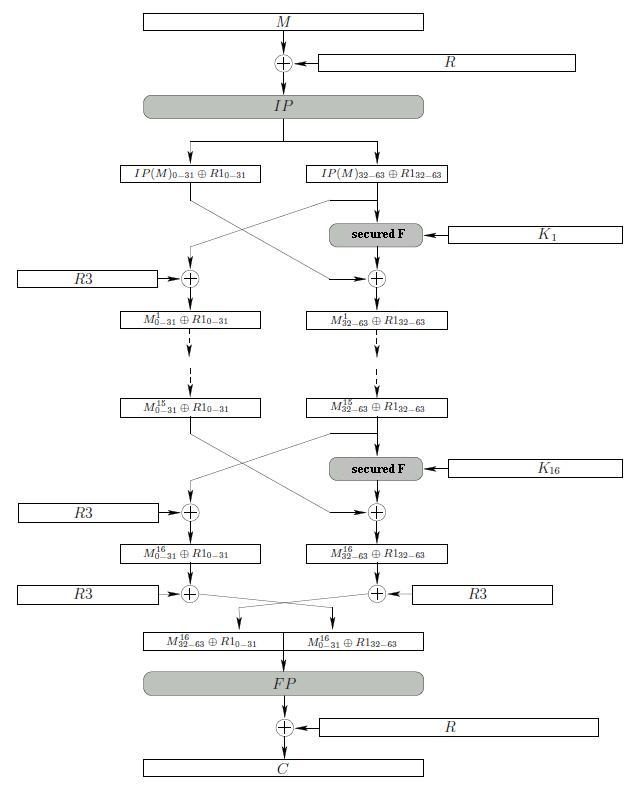
\includegraphics[scale=1.15]{images/dessecured.jpg}\\
\textit{Secured DES general scheme}
\end{center}
\newpage

\paragraph*{}
Note, that those pre-computation have to be computed in a very safe way.
Indeed, if an attacker could know those values, then immediately she/he could 
anticipate the SM-boxes for each encryption, therefore they would just launch a DPA 
attack simply changing the S boxes for the SM-boxes at each encryption.

\begin{center}
$SM(X)=S(X \oplus R2) \oplus P^{-1}( R3)$
\end{center}

\paragraph*{}
The algorithm has to be modified so as to the mask no to enter in the Sbox.
We obtain before the S-Box a intermediary value masked with $R2$. And clearly with this with 
new definition of the Sbox if the input is masked with $R_2$ 
then $R_2$ absolutely does not influence the output of those modified SMbox.


\begin{center}
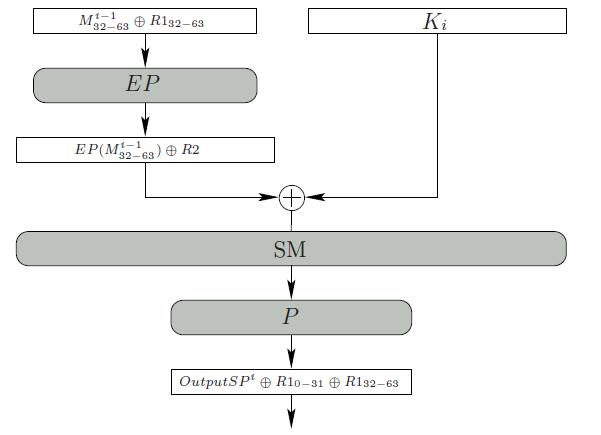
\includegraphics[width=110mm]{images/functionFsecured.jpg}\\
\textit{Secured F function}
\end{center}


\subsubsection{A round with a secured DES}

\paragraph*{} Here will be presented a complete round with the secured DES, 
and we will see that that at the end of a round the difference between a normal DES and 
the secured DES is always constant and worth $IP(R)$.
\vspace{5mm}

\textbf{Here} the letter $M$ is redefined for $M^i$ with the following convention
\begin{itemize}
\item $M^0$ stands fir the plain-text.
\item $\forall \in [1,16], \; M^i$ stand for the left|right value at the beginning
of the $i^{th}$ round.
\item $M^{17}$ stands fir the plain-text.
\end{itemize}

First of all, let's recall what is the output of this round DES algorithm, 
if we concatenate the two part, we have :
\begin{center}
$DesLeft | DesRight = M_{32-63}^i  |  P(S(EP(M_{32-63}^i) \oplus K_{i})))\oplus M_{0-31}^i$
\end{center}
Starting \footnote{In fact this lines are the induction step of a recurrence proof}
at the beginning of a round, noted $ i $, let's first calculate the 
result at the end of this round for the left side:\\
$SecuredLeft_i=M_{0-31}^i \oplus R1_{0-31}$ \\
$SecuredLeft^{'} = M_{32-63}^i \oplus R1_{32-63} \oplus R3 $ \\ 
$SecuredLeft_{i+1} = M_{32-63}^i \oplus R1_{0-31} $ \\
Secondly the same computation will be done on the right side:\\
$SecuredRight_i = M_{32-63}^i \oplus R1_{32-63} $ \\ 
$SecuredRight^{'} = EP(M_{32-63}^i) \oplus EP(R1_{32-63}) $ \\ 
$SecuredRight^{'} = EP(M_{32-63}^i) \oplus EP(R1_{32-63}) \oplus R2   $ \\ 
$SecuredRight^{'} = EP(M_{32-63}^i) \oplus K_{i} $ \\ 
$SecuredRight^{'} = 
S(EP(M_{32-63}^i) \oplus K_{i})) \oplus P^{-1}( R1_{0-31}\oplus R1_{32-63}) $ \\ 
$SecuredRight^{'} = 
P(S(EP(M_{32-63}^i) \oplus K_{i}))) \oplus R1_{0-31}\oplus R1_{32-63} $ \\ 
$SecuredRight_{i+1}= 
P(S(EP(M_{32-63}^i) \oplus K_{i})))\oplus M_{0-31}^i \oplus R1_{32-63}$ 
\vspace{5mm}
\begin{center}
$SecuredLeft_i | SecuredRight_i
	= M_{32-63}^i \oplus R1_{0-31} 
	| P(S(EP(M_{32-63}^i) \oplus K_{i})))\oplus M_{0-31}^i \oplus R1_{32-63}	$ \\
\end{center}



As a result we can see that the result, which explain that the variable obtained at the
end of a round a secured DES is the same than the one obtained by a normal DES Xored by $R1$:
\begin{center}
$SecuredLeft_i | SecuredRight_i = DesLeft_i| DesRight_i \oplus R1$\\
\end{center}

\subsubsection{Resistance against the first order DPA}
\paragraph*{} As we could see all the sensible variables of the secured DES are masked, 
moreover this boolean random mask has a uniform distribution.\\

\vspace{3mm}
With the following lemma :\\
\textbf{\textit{Let $\alpha$ $\in$ ${\mathbb{F}_2}^{n}$ an independent variable and
 $\beta$ another variable distributed uniformly on ${\mathbb{F}_2}^{n}$ and
  independent with $\alpha$. The variable $\alpha \oplus \beta$ is
 distributed uniformly and is independent with $\alpha$.}}\\
 \\
\indent Consequently we can deduct that all the variable which are manipulated
during the execution of the algorithm are uniformly distributed and
independent with the input and the key round. Thus this method resist against the
attacks of the first order DPA.


\subsubsection{Practical implementation}

In fact if the transforming masking method clearly prevent DPA attacks, 
-see before- it is not immune against side channel attacks
-see \ref{The_superposition_attack}-.
Therefore, this implementation can not be considered as secure anymore.
But in fact the "The superposition attack" can be prevented quick easily in fact:
we just have to forbid the superposition of the curve of 1st and 16th round.
This is why this Protected DES can be used at the condition to use 
two set of SM-box (one for round 1 to 8 and another for round 8 to 16).
In this configuration it is a quite popular implementation.

